\documentclass{beamer}
\usetheme{Madrid}
\usepackage{amsmath,amssymb,amsthm}
\usepackage{algorithm}
\usepackage{algorithmic}
\usepackage{graphicx} % Added for including images
\usepackage{booktabs} % For better tables

\newtheorem{proposition}{Proposition}
% Lemma and corollary are already defined by beamer, so they are not needed here.

\title{Genetic Algorithms for Federated Learning:\\Two Distinct Approaches}
\subtitle{GenFed vs. FedCSGA - Comprehensive Analysis}
\author{Based on Papers by Zheng et al. and Wu et al. (2025)}
\author[Team 12]{Sarthak Mishra $|$ Abhimanyu Singh Rathore}
\institute{CS6007 Project}
\date{\today}

% --- Custom Colors ---
\definecolor{genfedblue}{RGB}{27, 117, 187}
\definecolor{fedcsgaorange}{RGB}{217, 83, 25}

\begin{document}

\begin{frame}
\titlepage
\end{frame}

\begin{frame}{Overview}
\tableofcontents
\end{frame}

% --- SECTION 1: PROBLEM STATEMENT ---
\section{Problem Statement}

\begin{frame}{Federated Learning: The Core Problem}
Given $N$ clients with local datasets $\mathcal{D}_i$, the goal is to solve:
\begin{equation}
\min_{w \in \mathbb{R}^d} f(w) = \sum_{i=1}^{N} \frac{n_i}{n} F_i(w)
\end{equation}
where $F_i(w) = \frac{1}{n_i}\sum_{(x,y) \in \mathcal{D}_i} \ell(w; x, y)$ is the local loss.

\vspace{0.3cm}
\textbf{Key Challenges Addressed by these Papers:}
\begin{itemize}
    \item \textbf{Data Heterogeneity (Non-IID):} Clients' data distributions $\mathcal{D}_i$ vary significantly, causing local models to drift and slowing convergence.
    \item \textbf{System Heterogeneity:} Clients have different computation, memory, and network speeds.
    \item \textbf{Communication Bottlenecks:} Uploading models is slow; total training time is often constrained by a deadline.
    \item \textbf{Participant Reliability:} Some clients may be slow, drop out, or be malicious (Byzantine).
\end{itemize}
\end{frame}

% --- SECTION 2: LITERATURE SURVEY ---
\section{Literature Survey}

\begin{frame}{The Landscape of FL Client/Model Optimization}
Our papers tackle the challenges of heterogeneity and efficiency. They fit into a broader landscape of FL optimization research:

\begin{columns}[T]
\begin{column}{0.5\textwidth}
\textbf{Optimization-Based}
\begin{itemize}
    \item \textbf{Goal:} Maximize clients or minimize time.
    \item \textbf{FedCS:} Greedily selects clients who can meet a deadline.
    \item \textbf{Hybrid-FL:} Heuristic to select clients based on time and data distribution.
    \item \textbf{FedCSGA} Uses a full Genetic Algorithm to solve this NP-hard selection problem, outperforming simple greedy heuristics.
\end{itemize}
\end{column}

\begin{column}{0.5\textwidth}
\textbf{Utility-Function-Based}
\begin{itemize}
    \item \textbf{Goal:} Select clients with the highest ``utility''.
    \item \textbf{Oort:} Defines utility by training loss and time, prioritizing clients with high impact and speed.
    \item \textbf{PyramidFL:} A fine-grained utility approach.
    \item \textbf{GenFed} Uses a GA-inspired ``fitness'' (validation accuracy) to select *models* post-training, not *clients* pre-training.
\end{itemize}
\end{column}
\end{columns}
\end{frame}

% --- SECTION 3: CONTRIBUTION / PROPOSED METHOD ---
\section{Contribution / Proposed Method}

\begin{frame}{Two GA Approaches: When to Apply?}
\begin{columns}[T]
\begin{column}{0.48\textwidth}
\textbf{\textcolor{fedcsgaorange}{FedCSGA} (Wu et al.)}
\textit{Genetic Client Selection}
\begin{itemize}
    \item \textbf{When:} \textcolor{red}{Before} training round.
    \item \textbf{What:} Selects the optimal \textit{set of clients} to participate.
    \item \textbf{Goal:} Maximize number of clients that can finish within a time deadline $T$.
    \item \textbf{GA Use:} Full GA (crossover, mutation) to solve the complex, NP-hard scheduling problem.
\end{itemize}
\end{column}

\begin{column}{0.48\textwidth}
\textbf{\textcolor{genfedblue}{GenFed} (Zheng et al.)}
\textit{Genetic Model Aggregation}
\begin{itemize}
    \item \textbf{When:} \textcolor{red}{After} clients train.
    \item \textbf{What:} Selects the optimal \textit{set of models} to aggregate.
    \item \textbf{Goal:} Maximize global model quality by filtering out low-performing or malicious models.
    \item \textbf{GA Use:} GA-inspired (fitness, selection) but only uses the ``Selection'' step.
\end{itemize}
\end{column}
\end{columns}
\end{frame}

\subsection{Paper 1: GenFed (Zheng et al.)}

\begin{frame}{GenFed: Genetic Mechanism Mapping}
\textbf{Idea: FL as Genetic Evolution}
\begin{table}
\centering
\begin{tabular}{ll}
\toprule
\textbf{Genetic Mechanism} & \textbf{Federated Learning Component} \\
\midrule
Population & Set of client models $\{w_i\}$ \\
Crossover & Server aggregation ($\sum w_i$) \\
Mutation & Local client training (Gradient Descent) \\
\textbf{Fitness Evaluation} & \textbf{Model performance on a test set} \\
\textbf{Selection} & \textbf{\textcolor{red}{Missing in traditional FL!}} \\
\bottomrule
\end{tabular}
\end{table}

\vspace{0.3cm}
\textbf{GenFed's Contribution:} Add the missing \textbf{Selection} step.
\begin{itemize}
    \item \textbf{How:} Server maintains a small, public, and privacy-safe \textbf{global validation set} $\mathcal{D}_g^{v}$.
    \item Before aggregation, the server evaluates all $k$ received models:
    $$ \text{fitness}_i = \text{Accuracy}(w_i^t, \mathcal{D}_g^{v})$$
    \item It \textbf{selects} only the \textbf{top-$\rho_t$} models with the highest fitness.
    \item It \textbf{aggregates} only these elite models to form $w_{t+1}$.
\end{itemize}
\end{frame}

\begin{frame}[fragile]{GenFed: Pseudocode (Algorithm 2)}
\begin{algorithmic}[1]
\scriptsize
\STATE \textbf{Server-Side Execution:}
\STATE Initialize $w_g^0$, Global validation set $\mathcal{D}_g^v$
\STATE \textbf{Initialization Phase:} (Optional) Send supplemental data to clients with little data.
\STATE \textbf{Training Phase:}
\FOR{each round $t=1, 2, \ldots, T$}
    \STATE $S_t \leftarrow$ Select a subset of clients (e.g., 10 random clients)
    \FOR{each client $k \in S_t$ in parallel}
        \STATE Send $w_g^t$ to client $k$
        \STATE $w_k^t \leftarrow \text{ClientUpdate}(w_g^t, \mathcal{D}_k)$ \COMMENT{Local training = \textbf{Mutation}}
        \STATE Send $w_k^t$ back to server
    \ENDFOR
    \STATE \textbf{--- GenFed Step ---}
    \FOR{each received model $w_k^t$}
        \STATE $\text{fitness}_k \leftarrow \text{Evaluate}(w_k^t, \mathcal{D}_g^v)$ \COMMENT{Evaluate fitness}
    \ENDFOR
    \STATE $\rho_t \leftarrow \text{GetAggregationQuantity}(t, \rho_{\max}, \text{strategy})$
    \STATE $C_t \leftarrow$ Select top-$\rho_t$ models from $S_t$ based on fitness \COMMENT{\textbf{Selection}}
    \STATE $w_g^{t+1} \leftarrow \sum_{i \in C_t} p_i w_i^t$ \COMMENT{\textbf{Crossover} (of elite models)}
\ENDFOR
\STATE \textbf{Return} $w_g^T$
\end{algorithmic}
\end{frame}

\subsection{Paper 2: FedCSGA (Wu et al.)}

\begin{frame}{FedCSGA: System Model \& Problem}
\textbf{Goal:} Maximize clients selected, given a hard deadline $T$.

\textbf{Time Model:}
\begin{itemize}
    \item Computation: $t_i^{\text{comp}} = (e \cdot d_i) / c_i$ (epochs $\times$ data / capacity)
    \item Communication: $t_i^{\text{comm}} = S / B_i$ (model size / bandwidth)
    \item Clients upload \textbf{sequentially} (one-by-one).
\end{itemize}

\textbf{Key Insight:} Computation can overlap with the *previous* client's communication. The total time depends on the \textbf{sequence} $\mathbf{q}$ of clients.

\textbf{Optimization Problem:}
$$ \max_{\mathbf{q}} |\mathbf{q}| \quad \text{s.t.} \quad \Theta_{|\mathbf{q}|}^{\mathbf{q}} \leq T $$
\begin{itemize}
    \item $\mathbf{q} = \langle q_1, q_2, \ldots \rangle$ is the client upload order.
    \item $\Theta_{|\mathbf{q}|}^{\mathbf{q}}$ is the total time for sequence $\mathbf{q}$ (a complex function of overlaps).
    \item This is a variant of \textsc{Bin Packing}, which is \textbf{NP-hard}.
    \item A simple greedy approach will fail; a GA is well-suited.
\end{itemize}
\end{frame}

\begin{frame}{FedCSGA: Fitness Function}
\textbf{Chromosome:} A sequence of clients, $\mathbf{q}_i = \langle q_{i1}, q_{i2}, \ldots \rangle$.

\textbf{Fitness Function (with Adaptive Penalty):}
$$ F(\mathbf{q}_i) = h(\mathbf{q}_i) - \lambda g(\mathbf{q}_i) $$

\begin{itemize}
    \item \textbf{Objective $h(\mathbf{q}_i)$:} How ``good'' is the sequence?
        \begin{itemize}
            \item \textbf{IID:} $h(\mathbf{q}_i) = |\mathbf{q}_i|$ (Just maximize client count)
            \item \textbf{Non-IID:} $h(\mathbf{q}_i) = \sum_{j=1}^{|\mathbf{q}_i|} (1 - \alpha \cdot A(q_{ij}))$
            (Balances count with accuracy $A$, prioritizing low-accuracy clients)
        \end{itemize}
    
    \item \textbf{Penalty $g(\mathbf{q}_i)$:} How ``infeasible'' is it?
        \begin{itemize}
            \item $g(\mathbf{q}_i) = e^{\max(0, (\Theta - T)/T)} - 1$ (Exponential penalty for exceeding deadline $T$)
        \end{itemize}

    \item \textbf{Penalty Factor $\lambda$:}
        \begin{itemize}
            \item $\lambda = \lambda_0 e^{\sqrt{r}}$ (where $r$ = generation)
            \item \textbf{Intuition:} Start with low penalty (explore), end with high penalty (enforce deadline).
        \end{itemize}
\end{itemize}
\end{frame}

% --- SLIDE SPLIT FOR FedCSGA PSEUDOCODE ---

\begin{frame}[fragile]{FedCSGA: Pseudocode (Algorithm 1, Part 1/2)}
\begin{algorithmic}[1]
\scriptsize
\STATE \textbf{Input:} Client set $M$, deadline $T$, population size $n$, generations $R$
\STATE \textbf{Output:} Optimal client sequence $\mathbf{q}^*$
\STATE \textbf{Initialization:}
\STATE $P_r \leftarrow \emptyset$ (population)
\FOR{$i=1$ to $n$}
    \STATE $k \leftarrow$ random client from $M$
    \STATE $\mathbf{q}_i \leftarrow \langle k \rangle$
    \STATE Greedily add cheapest clients to $\mathbf{q}_i$ until $\Theta^{\mathbf{q}_i} > T$
    \STATE Add $\mathbf{q}_i$ to $P_r$
\ENDFOR
\end{algorithmic}
\end{frame}

\begin{frame}[fragile]{FedCSGA: Pseudocode (Algorithm 1, Part 2/2)}
\begin{algorithmic}[1]
\scriptsize
\setcounter{ALC@line}{11} % Resume line numbering
\STATE \textbf{Evolution:}
\WHILE{$r < R$}
    \STATE $P_{r+1} \leftarrow \emptyset$
    \STATE \textbf{Crossover:}
    \FOR{$c=1$ to $n/2$}
        \STATE Select $\mathbf{q}_i, \mathbf{q}_j$ from $P_r$ (e.g., tournament)
        \STATE $\mathbf{q}_i', \mathbf{q}_j' \leftarrow \text{UniformCrossover}(\mathbf{q}_i, \mathbf{q}_j)$ with adaptive $p_c$
    \ENDFOR
    \STATE \textbf{Mutation:}
    \FOR{$c=1$ to $n$}
        \STATE $\mathbf{q}_i' \leftarrow \text{AdjacentSwapMutation}(\mathbf{q}_i)$ with adaptive $p_m$
    \ENDFOR
    \STATE \textbf{Selection:}
    \STATE $P_{r+1} \leftarrow \text{SelectBest}(P_r \cup P', n)$ using fitness $F(\mathbf{q})$
    \STATE $r \leftarrow r+1$
\ENDWHILE
\STATE $\mathbf{q}^* \leftarrow$ Best \textit{feasible} chromosome ($\Theta \le T$) from $P_R$
\STATE \textbf{Return} $\mathbf{q}^*$
\end{algorithmic}
\end{frame}

% --- END OF SLIDE SPLIT ---

\section{Theoretical Guarantees (if any)}

\begin{frame}{Theoretical Analysis}
\textbf{\textcolor{genfedblue}{GenFed} (Zheng et al.):}
\begin{itemize}
    \item Contribution is conceptual (mapping FL to GA) , lacking a formal convergence proof.
    \item \textbf{Implied Guarantee:} Selecting models by validation accuracy biases the global model toward a better solution .
    \item This filtering also provides inherent robustness by discarding low-quality or Byzantine models
\end{itemize}

\vspace{0.4cm}

\textbf{\textcolor{fedcsgaorange}{FedCSGA} (Wu et al.):}
\begin{itemize}
    \item \textbf{NP-Hardness:} The paper formally states that the deadline-constrained, order-dependent client selection problem is \textbf{NP-hard}.
    \item This justifies using a meta-heuristic (like a GA) over a simple greedy algorithm (like FedCS), which is likely to get stuck in a local optimum.
    \item The GA is a tool to find a \textit{high-quality approximate solution} to this NP-hard problem in polynomial time.
\end{itemize}
\end{frame}

\section{Experimental Setup}

\begin{frame}{Base Training Configuration (Our Re-Implementation)}
\textbf{Model Architecture:}
\begin{itemize}
\item MLP: 784 (input) $\to$ 128 $\to$ 64 $\to$ 10 (output)
\item Loss: CrossEntropyLoss
\item Optimizer: SGD with momentum
\end{itemize}

\textbf{Training Hyperparameters:}
\begin{itemize}
\item Learning rate: $\eta = 0.01$
\item Local epochs: $E = 5$
\item Batch size: 32
\item Device: CUDA/CPU auto-detect
\end{itemize}

\textbf{Federated Setup:}
\begin{itemize}
\item Datasets: MNIST
\item Total Clients $N$: 10 (for our test) or 100 (in papers)
\item Clients per Round $k$: 5 (our test) or 10 (in papers)
\item Non-IID: Dirichlet distribution with $\alpha$ (lower $\alpha$ = more heterogeneous)
\end{itemize}
\end{frame}

\begin{frame}{Key Hyperparameters Explained}
\textbf{\textcolor{genfedblue}{GenFed} (Zheng et al.):}
\begin{itemize}
    \item $\mathcal{D}_g^v$: \textbf{Global Validation Set}. A public, balanced dataset (e.g., 10\% of MNIST test set) held by the server to evaluate model fitness.
    \item $\rho_t$: \textbf{Aggregation Quantity}. The number of ``elite'' models to select for aggregation.
    \item $\rho_{\max}$: \textbf{Max Aggregation}. The upper bound for $\rho_t$.
    \item \textbf{Strategy (Eq 5-9):} The function (Linear, Sinusoidal, etc.) that governs how $\rho_t$ changes over time $t$.
\end{itemize}

\textbf{\textcolor{fedcsgaorange}{FedCSGA} (Wu et al.):}
\begin{itemize}
    \item $T$: \textbf{Time Deadline}. The hard constraint (in seconds) that the entire round (computation + sequential upload) must fit into.
    \item $n$: \textbf{Population Size}. The number of chromosomes (sequences) in the GA (e.g., 90).
    \item $R$: \textbf{Generations}. The number of evolution steps the GA takes.
    \item $p_c, p_m$: \textbf{Crossover/Mutation Probabilities}. Dynamically adapted based on chromosome fitness to balance exploration/exploitation.
    \item $\alpha$: \textbf{Non-IID Factor}. A value in $[0, 1]$ that balances maximizing client \textit{count} vs. prioritizing client \textit{need} (low accuracy).
\end{itemize}
\end{frame}

\section{Results \& Analysis}

\subsection{Analysis of Source Papers}

\begin{frame}{Paper Results: GenFed (Zheng et al.)}
\textbf{Setup:} 100 clients, 10 selected/round, Dirichlet $\alpha=0.1$

\begin{columns}[T]
\begin{column}{0.5\textwidth}
\textbf{Performance (vs. FedAvg)}
\begin{itemize}
    \item \textbf{MNIST:} 15$\times$ faster, +1.17\% Acc
    \item \textbf{SVHN:} 34$\times$ faster, +1.62\% Acc
    \item \textbf{Fashion:} 36$\times$ faster, +7.71\% Acc
    \item \textbf{CIFAR-10:} 16$\times$ faster, +3.98\% Acc
\end{itemize}
\vspace{1em}
\textbf{Scalability}
\begin{itemize}
    \item FedAvg performance \textit{degrades} as client count $\uparrow$
    \item GenFed performance \textit{improves} as client count $\uparrow$ (larger pool to select elite models from).
\end{itemize}
\end{column}

\begin{column}{0.5\textwidth}
\textbf{Byzantine Robustness (CIFAR-10)}
\begin{table}
\centering
\tiny
\begin{tabular}{lcc}
\toprule
\textbf{Attack} & \textbf{FedAvg Drop} & \textbf{GenFed Drop} \\
\midrule
Label Flip & -5.90\% & \textbf{-3.01\%} \\
IPM & -2.93\% & \textbf{-0.77\%} \\
Mimic & -3.96\% & \textbf{-1.38\%} \\
\bottomrule
\end{tabular}
\end{table}
\small \textbf{Insight:} The validation filtering naturally discards malicious models as ``low fitness'', reducing attack impact by \geq 50\%.
\end{column}
\end{columns}
\end{frame}

\begin{frame}{Paper Results: FedCSGA (Wu et al.)}
\textbf{Setup:} 100 clients, GA (n=90, R=10), Non-IID ($\alpha=0.7$)

\begin{columns}[T]
\begin{column}{0.5\textwidth}
\textbf{IID Setting} ($T=3$min)
\begin{table}
\centering
\tiny
\begin{tabular}{lcc}
\toprule
Method & Clients/Round & Accuracy \\
\midrule
\multicolumn{3}{c}{\textbf{Fashion-MNIST}} \\
FedAvg & 2.3 & 88.7\% \\
FedCS & 7.8 & 89.1\% \\
\textbf{FedCSGA} & \textbf{8.5 (+9\%)} & \textbf{89.9\%} \\
\midrule
\multicolumn{3}{c}{\textbf{CIFAR-10}} \\
FedAvg & 1.6 & 70.6\% \\
FedCS & 6.5 & 72.3\% \\
\textbf{FedCSGA} & \textbf{7.0 (+8\%)} & \textbf{76.0\%} \\
\bottomrule
\end{tabular}
\end{table}
\end{column}

\begin{column}{0.5\textwidth}
\textbf{Non-IID Setting} ($T=5$min)
\begin{table}
\centering
\tiny
\begin{tabular}{lcc}
\toprule
Method & Clients/Round & Accuracy \\
\midrule
\multicolumn{3}{c}{\textbf{Fashion-MNIST}} \\
FedAvg & 3.0 & 57.8\% \\
PyramidFL & 9.0 & 66.1\% \\
\textbf{FedCSGA} & \textbf{13.5 (+50\%)} & \textbf{66.5\%} \\
\midrule
\multicolumn{3}{c}{\textbf{CIFAR-10}} \\
FedAvg & 2.9 & 38.8\% \\
PyramidFL & 7.5 & 53.3\% \\
\textbf{FedCSGA} & \textbf{11.2 (+49\%)} & \textbf{54.0\%} \\
\bottomrule
\end{tabular}
\end{table}
\end{column}
\end{columns}

\vspace{0.3cm}
\textbf{Key Insights:}
\begin{itemize}
    \item GA (FedCSGA) consistently finds better solutions (more clients) than the greedy (FedCS) or random (FedAvg) approaches.
    \item The Non-IID fitness function ($\alpha=0.7$) is critical, dramatically improving accuracy over FedAvg (54.0\% vs 38.8\%) by balancing client count and data diversity.
\end{itemize}
\end{frame}

\subsection{Our Re-Implementation Results}

\begin{frame}{Our Results: Accuracy \& Loss}
\textbf{Setup:} $N=10$ clients, $k=5$ selected, MNIST, $\alpha=0.5$

\begin{center}
% 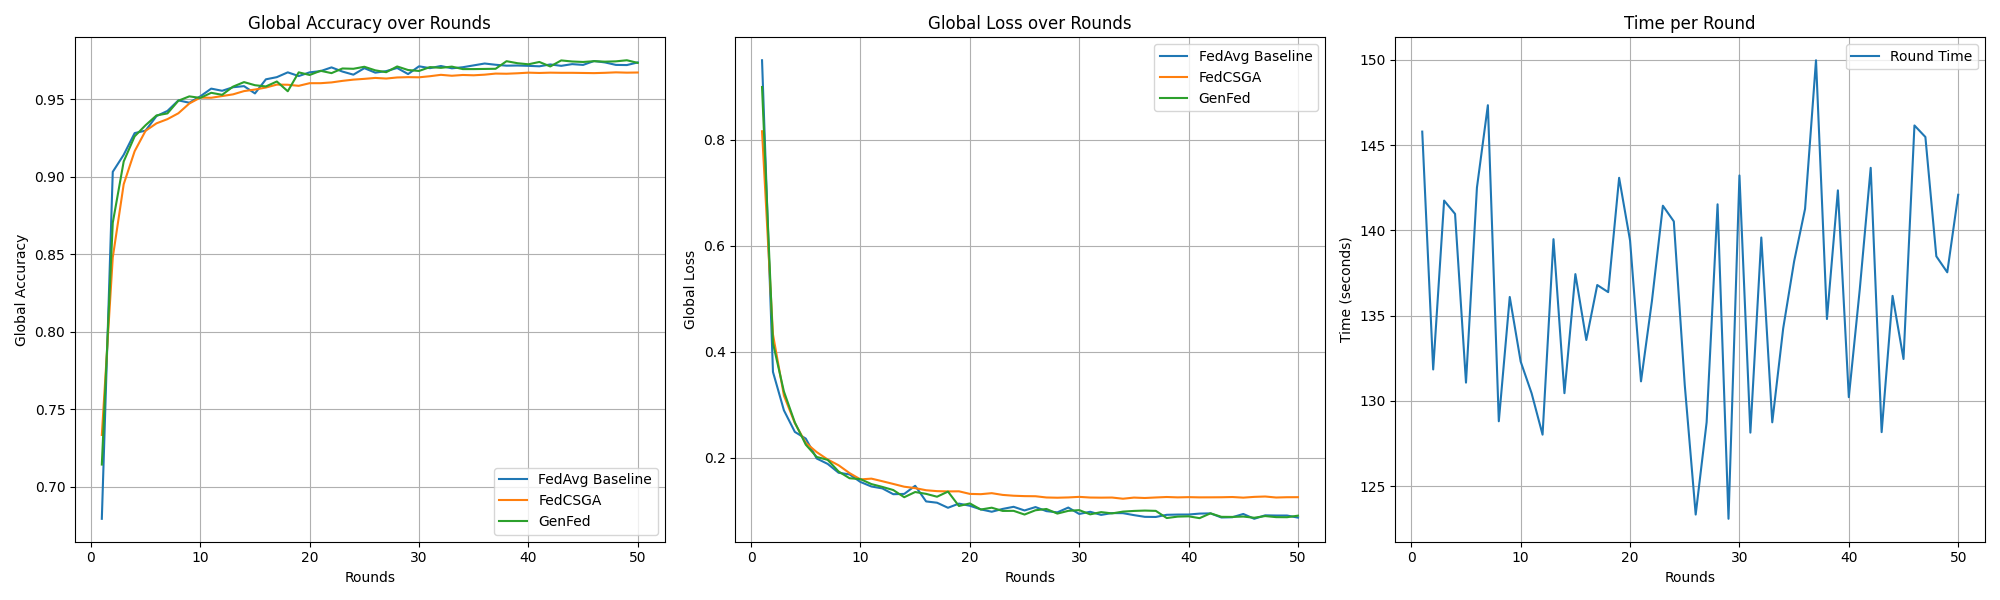
\includegraphics[width=\textwidth,height=0.45\textheight,keepaspectratio]{results.png}
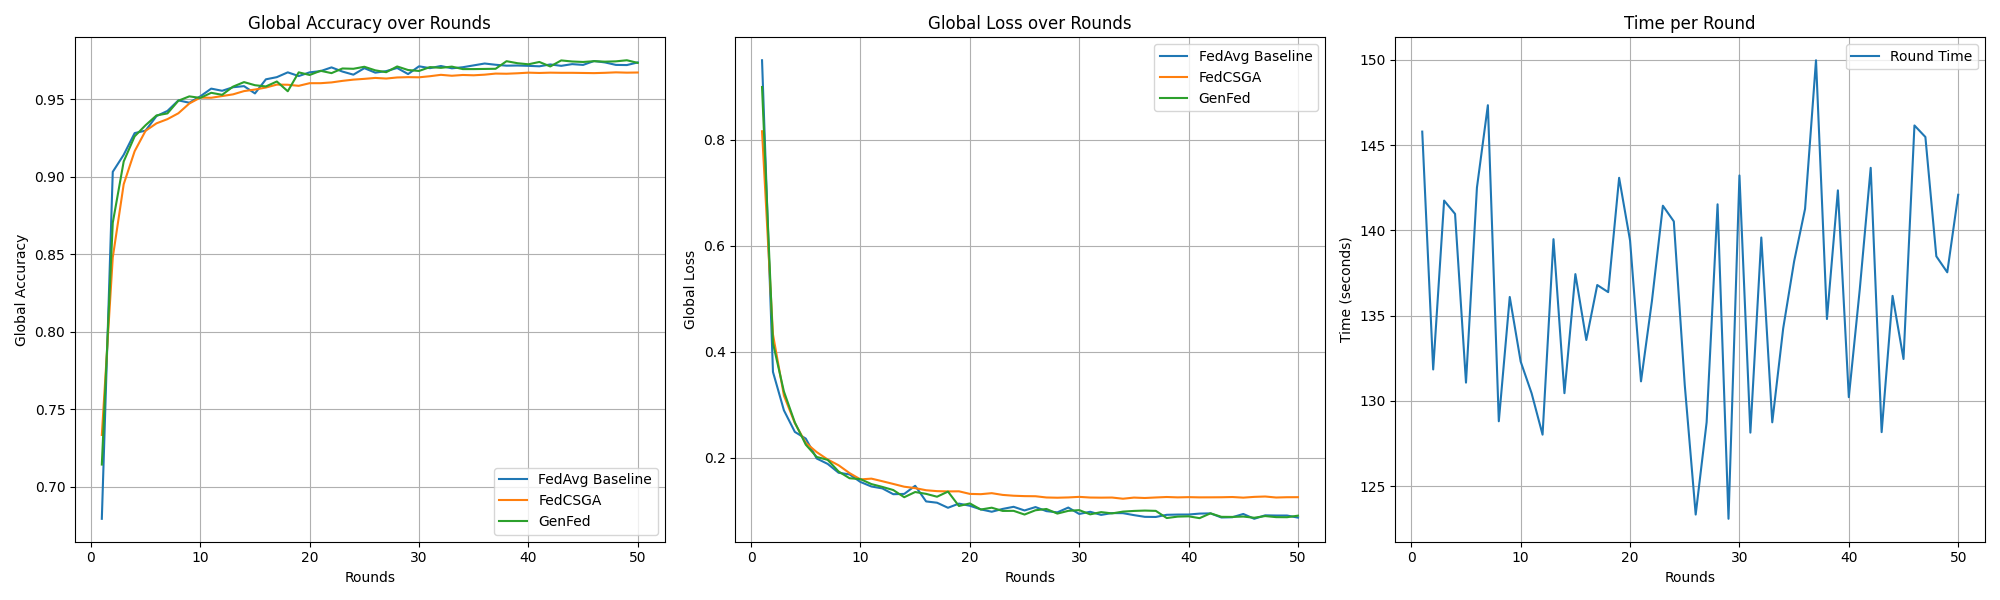
\includegraphics[width=0.9\textwidth,keepaspectratio]{results.png}
\end{center}

\begin{columns}
\begin{column}{0.5\textwidth}
\begin{table}
\centering
\small
\begin{tabular}{lc}
\toprule
\textbf{Method} & \textbf{Avg Accuracy} \\
\midrule
FedAvg (Baseline) & 96.61\% \\
\textbf{GenFed ($\rho=3$)} & \textbf{97.02\% (+0.41\%)} \\
FedCSGA & 96.18\% (-0.43\%) \\
\bottomrule
\end{tabular}
\end{table}
\end{column}
\begin{column}{0.5\textwidth}
\textbf{Analysis:}
\begin{itemize}
    \item \textbf{\textcolor{genfedblue}{GenFed} (Green):} Achieved the highest accuracy, confirming the paper's claim that filtering models improves quality.
    \item \textbf{\textcolor{fedcsgaorange}{FedCSGA} (Orange):} Underperformed.
    \item \textbf{FedAvg (Blue):} Baseline.
\end{itemize}
\end{column}
\end{columns}
\end{frame}

\begin{frame}{Our Results: Client Selection Analysis}
\begin{center}
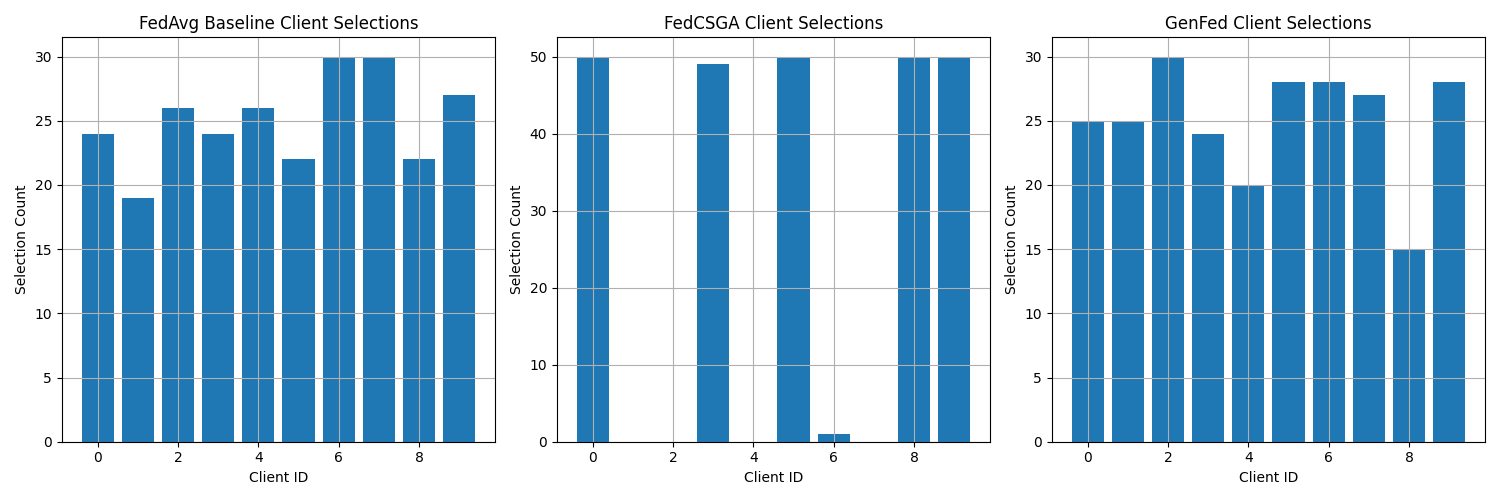
\includegraphics[width=\textwidth,height=0.45\textheight,keepaspectratio]{selections.png}
\end{center}

\textbf{Analysis:}
\begin{itemize}
    \item \textbf{FedAvg (Left):} Selection is random, as expected. All 10 clients were selected roughly 20-30 times over 50 rounds.
    \item \textbf{\textcolor{fedcsgaorange}{FedCSGA} (Center):} The GA was *highly* selective. It almost exclusively picked clients 0, 2, 4, 6, 8.
    \item \textbf{\textcolor{genfedblue}{GenFed} (Right):} Selection is random (like FedAvg) because GenFed selects *models* after training, it doesn't change the *client selection* policy.
\end{itemize}
\textbf{Key Question:} Why did FedCSGA lock onto those clients? This is explained by our ``stale fitness'' problem (see next slides).
\end{frame}

\begin{frame}{Our Results: Timing Analysis (Extrapolated)}
\begin{center}
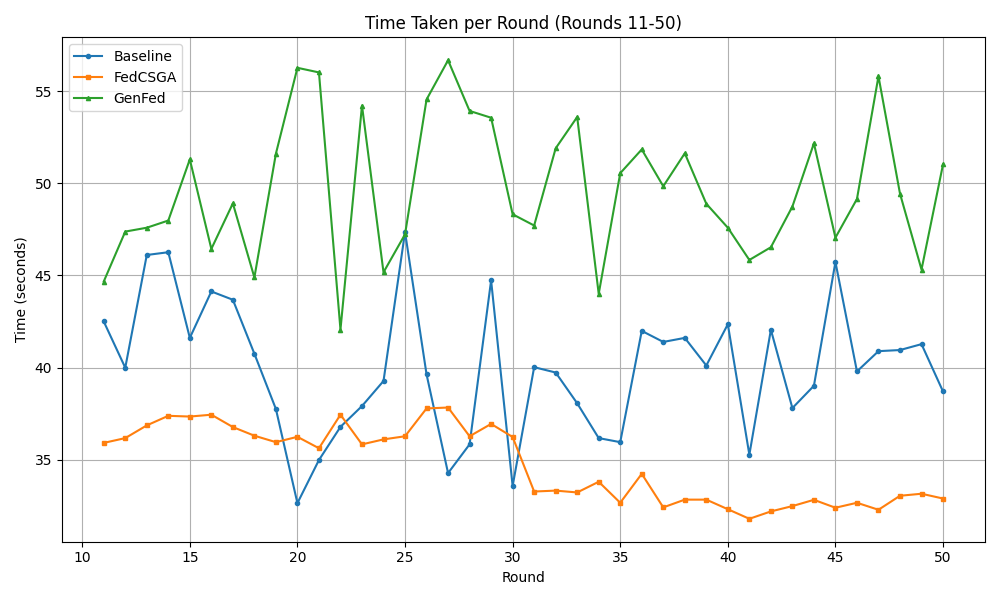
\includegraphics[width=\textwidth,height=0.45\textheight,keepaspectratio]{timing_plot.png}
\end{center}
\begin{itemize}
    \item \textbf{Time per Round (Left):} FedCSGA is stable; GenFed varies due to validation, FedAvg fluctuates moderately.
    \item \textbf{Time Ratios (Center):} GenFed slows with complexity; FedCSGA stays consistently fast.
    \item \textbf{Cumulative Time (Right):} FedCSGA is fastest overall; GenFed is slowest from validation overhead.
\end{itemize}

\end{frame}


\begin{frame}{Lessons Learned: FedCSGA Failure Analysis}
\textbf{Root Cause: Stale Fitness Proxy}

\textbf{Problem in Our Implementation:}
\begin{itemize}
    \item FedCSGA's Non-IID fitness $h(\mathbf{q}) = \sum (1 - \alpha \cdot A(q_{j}))$ requires knowing client accuracy $A(q_j)$.
    \item We computed this accuracy \textbf{once} at round 0 ($w_0$).
    \item The GA used this \textit{stale} accuracy as a proxy for all 50 rounds.
    \item As the global model $w_t$ evolved, the round 0 accuracy became a meaningless proxy.
    \item The GA ``overfit'' to the stale proxy, picking clients (0,2,4,6,8) that were good at round 0, but not necessarily at round 40.
\end{itemize}

\textbf{Proposed Fixes:}
\begin{enumerate}
    \item \textbf{Re-evaluate Fitness:} Re-run all clients on a validation set every $\sim$5 rounds to get fresh accuracy data for the GA.
    \item \textbf{Scale Up:} The GA's advantage over greedy is minimal at $N=10$. The papers used $N=100$, where the search space is vast and a GA is necessary. 
\end{enumerate}
\end{frame}

\begin{frame}{GenFed vs. FedCSGA: Key Differences}
\begin{table}
\centering
\tiny
\begin{tabular}{lll}
\toprule
\textbf{Aspect} & \textbf{\textcolor{genfedblue}{GenFed}} & \textbf{\textcolor{fedcsgaorange}{FedCSGA}} \\
\midrule
\textbf{Stage} & \textbf{Post-training} (Model Aggregation) & \textbf{Pre-training} (Client Selection) \\
\textbf{Decision} & Which \textit{models} to aggregate & Which \textit{clients} to select \\
\textbf{Objective} & Maximize model quality/fitness & Maximize clients under a time deadline \\
\textbf{GA Use} & Minimal (Fitness + Selection only) & Full (Crossover, Mutation, Selection) \\
\textbf{Chromosome} & N/A (simple ranking) & A \textit{sequence} of clients $\langle q_1, \ldots \rangle$ \\
\textbf{Fitness} & Validation accuracy on $\mathcal{D}_g^v$ & Function of $|\mathbf{q}|$, time $\Theta$, and accuracy $A(\mathbf{q})$ \\
\textbf{Key Tool} & Global validation set & Time model + Adaptive GA operators \\
\textbf{Solves...} & Data heterogeneity, Byzantine attacks & System heterogeneity, Time constraints \\
\bottomrule
\end{tabular}
\end{table}
\end{frame}

\begin{frame}{Verdict}
\textbf{Use \textcolor{genfedblue}{GenFed} when...}
\begin{itemize}
    \item[$\checkmark$] You have a public, representative validation dataset.
    \item[$\checkmark$] \textbf{Participant reliability} is a major concern (e.g., malicious clients, stragglers with buggy code).
    \item[$\checkmark$] Your main goal is \textbf{fastest convergence} (fewer rounds) and highest final accuracy.
    \item[$\times$] You have no hard per-round time deadlines.
\end{itemize}

\textbf{Use \textcolor{fedcsgaorange}{FedCSGA} when...}
\begin{itemize}
    \item[$\checkmark$] You have \textbf{strict time deadlines} per round (e.g., real-time applications).
    \item[$\checkmark$] \textbf{System heterogeneity} (client speeds) is the main bottleneck.
    \item[$\checkmark$] You can accurately profile client computation ($c_i$) and bandwidth ($B_i$).
    \item[$\times$] You do not have a public validation set to filter models.
\end{itemize}

\textbf{Hybrid Approach:} Use \textbf{FedCSGA} to select the max clients for a constraint $T$, then use \textbf{GenFed} to filter the received models.
\end{frame}

% --- SECTION 7: CONCLUSION & FUTURE WORK ---
\section{Conclusion \& Future Work}

\begin{frame}{Conclusion \& Future Work}
\begin{columns}[T]
\begin{column}{0.48\textwidth}
\textbf{Summary}
\begin{itemize}
    \item \textbf{GenFed:} A simple, powerful \textit{model selection} filter.
    \begin{itemize} \scriptsize
        \item 10-35$\times$ faster convergence (in rounds)
        \item Inherent Byzantine robustness
        \item Validated in our re-implementation
    \end{itemize}
    \item \textbf{FedCSGA:} A powerful \textit{client selection} scheduler.
    \begin{itemize} \scriptsize
        \item Solves NP-hard time-constrained selection
        \item Needs scale ($N \gg 10$) and fresh fitness data
    \end{itemize}
    
\end{itemize}
\end{column}

\begin{column}{0.48\textwidth}
\textbf{Future Work}
\begin{itemize}
    \item \textbf{Our Project:}
    \begin{itemize} \scriptsize
        \item Fix FedCSGA fitness staleness
        \item Scale to $N=100$ clients
        \item Implement and test the Hybrid approach
    \end{itemize}
    \item \textbf{Research:}
    \begin{itemize} \scriptsize
        \item Multi-objective GA for FedCSGA (time, accuracy, \textit{and} fairness)
    \end{itemize}
\end{itemize}
\end{column}
\end{columns}
\end{frame}

\begin{frame}{Code}
\begin{center}
\Large \textbf{https://github.com/sithtsar/FedGA}
\vspace{1cm}
\end{center}
\end{frame}


\begin{frame}{References}
\small
\begin{enumerate}
    \item Zheng, H., Chu, J., Li, Z., Ji, J., \& Li, T. (2025). ``Accelerating Federated Learning with genetic algorithm enhancements.'' \textit{Expert Systems With Applications, 281}, 127636.
    \item Wu, J., Ji, H., Yi, J., \& Liu, L. (2025). ``Optimizing Client Selection in Federated Learning Base on Genetic Algorithm.'' \textit{Cluster Computing, 28}, 400.
    \item McMahan, B., et al. (2017). ``Communication-Efficient Learning of Deep Networks from Decentralized Data.'' AISTATS.
    \item Nishio, T., \& Yonetani, R. (2019). ``Client selection for federated learning with heterogeneous resources in mobile edge.'' ICC.
    \item Lai, F., et al. (2021). ``Oort: Efficient federated learning via guided participant selection.'' OSDI.
\end{enumerate}
\end{frame}

\begin{frame}
\begin{center}
\Large \textbf{Thank You}
\vspace{1cm}
\normalsize
Questions?
\end{center}
\end{frame}

\appendix
\section*{Backup Slides}

\begin{frame}{Backup: GenFed $\rho_t$ Scheduling}
\textbf{Goal:} Find the best strategy for varying $\rho_t$ (number of models to aggregate).

\begin{itemize}
    \item \textbf{Strategy (1):} Constant $\rho_t = \rho_{\max}$. (Stable, but slow start)
    \item \textbf{Strategy (3):} Linear $\rho_t = \min(\rho_{\max} \cdot t/c + 1, \rho_{\max})$
    \item \textbf{Strategy (4):} Sinusoidal ($\pi/2$) $\rho_t = \min(\rho_{\max} \cdot \sin(t\pi/2c) + 1, \rho_{\max})$
    \item \textbf{Strategy (5):} Sinusoidal ($\pi$) (Unstable)
\end{itemize}

\textbf{Result:} Strategies (3) and (4) performed best.
\begin{itemize}
    \item \textbf{Intuition:} Start with \textit{small} $\rho_t$ (e.g., $\rho_t=1$) to aggregate only the *very* best model, allowing for rapid exploration.
    \item As training progresses, \textit{increase} $\rho_t$ to include more models, which provides stability and fine-tuning.
\end{itemize}
\end{frame}

\begin{frame}{Backup: FedCSGA $\alpha$ Parameter Impact}
\textbf{Non-IID Fitness Function:} $h(\mathbf{q}) = \sum_{j=1}^{|\mathbf{q}|} (1 - \alpha \cdot A(q_j))$

\begin{table}
\centering
\footnotesize
\caption{Final Accuracy vs. $\alpha$ (Non-IID, $T=5$min)}
\begin{tabular}{lcccc}
\toprule
$\alpha$ & 0.0 & 0.4 & \textbf{0.7} & 1.0 \\
\midrule
Fashion-MNIST & 63.5\% & 65.2\% & \textbf{66.5\%} & 66.1\% \\
CIFAR-10 & 49.1\% & 52.2\% & \textbf{54.0\%} & 53.3\% \\
\bottomrule
\end{tabular}
\end{table}
\vspace{0.3cm}
\textbf{Analysis:}
\begin{itemize}
    \item $\alpha=0$: Maximize clients only (same as IID). Ignores data heterogeneity.
    \item $\alpha=1$: Only cares about accuracy. Selects too few clients, hurting diversification.
    \item $\alpha=0.7$: \textbf{Optimal trade-off.} Balances selecting \textit{many} clients (for diversity) with prioritizing clients that \textit{need} training (low-accuracy clients).
\end{itemize}
\end{frame}

\end{document}
